%-----------------------------------------------------------------------------
% Template for seminar 'Program Analysis' at TU Darmstadt.
%
% Adapted from template for sigplanconf LaTeX Class, which is a LaTeX 2e
% class file for SIGPLAN conference proceedings (by Paul C.
% Anagnostopoulos).
%
%-----------------------------------------------------------------------------


\documentclass[authoryear,preprint]{sigplanconf}

% A couple of packages that may be useful
\usepackage{amsmath}
\usepackage{amsfonts}
\usepackage{amssymb}
\usepackage{amsthm}
\usepackage{algorithm2e}
\usepackage{listings}
\usepackage{xcolor}
\usepackage{tikz}
\usepackage{booktabs}
\usepackage{subfigure}
\usepackage[english]{babel}
\usepackage{blindtext}
\usepackage[normalem]{ulem}

\begin{document}

\special{papersize=a4}
\setlength{\pdfpageheight}{\paperheight}
\setlength{\pdfpagewidth}{\paperwidth}


\title{System Dependence Graphs for Java Programs}

\authorinfo{Pavlos Milaszewicz}{}{}

\maketitle

\begin{abstract}
A System Dependence Graph (SDG) models inter-procedural data dependencies and control flow information within a program. SDGs can be thought of as an extension of a Program Dependence Graph (PDG), of which only models intra-procedural flow information; SDGs have extra branching sites to display the extraneous control flow arising from a method call. PDGs and SDGs have a number of practical uses, such as optimization, slicing, and debugging of software programs. Many program analysis toolkits, such as the Soot framework, provide built-in PDG generation features for Java programs, however, few exist that can automatically generate SDGs.    

In this paper we discuss our SDG implementation using the Soot framework. Soot can produce a PDG for any given target Java class; we extend this functionality by implementing a static analysis that detects function calls, and in which case, extra branches and nodes are added to the PDG, of which comprises the SDG. This is achieved by pre-generating the main PDG control flow, after which the graph is traversed for function calls.

We also discuss the results of the SDG implementation when pitted against sample Java programs. While we found that the analysis works somewhat correctly for ordinary function calls, more complex cases, such as anonymous functions and recursive calls, are not properly handled and so the analysis would need to be extended in the future to take into account these limitations.  
\end{abstract}


\section{Introduction}
\label{sec:introduction}

SDGs expand on the information provided by PDGs by allowing one to model inter-procedural control flows; the information within a function call is normally lost and/or disregarded in a normal PDG implementation. As such, SDGs have a significant advantage in that a more accurate representation of the system can be visualized, although with the price of increased complexity. 

Soot is a static analysis framework exclusively for Java programs. Since SDGs are a relatively newer concept in computer science, most frameworks do not provide a built-in SDG generator, including Soot. However, Soot is able to generate PDGs for a given Java class, which can be taken advantage of as SDGs are essentially a connected grouping of several PDGs.

The approach we take for the generation of SDGs are to extend the built-in SDG capabilities of Soot, wherein the final graph is a coalesced mesh of PDG graphs which are interconnected via the function entry and exit points.

\section{Soot PDGs}
\label{sec:some_section}

Soot provides off the shelf PDGs via the Soot Eclipse plugin. Note that an older Eclipse version (Kepler) and JDK/JRE 1.7 or lower environments are essential to make use of this functionality, as this seems to be a forgotten feature of Soot and is not at all maintained by the library authors; the PDG generation will not work with newer Eclipse and Java implementations, which is a significant drawback.

\subsection{Built-in PDG generation}

An example PDG is shown in Figure~\ref{f:sampPdg}. The analysis simply prints the local variables defined in the Java program shown in Figure~\ref{f:sampProg}. Notice that a function invocation in a Soot PDG is simply treated as just another node in the graph.

\begin{figure}[ht]
	\centering
	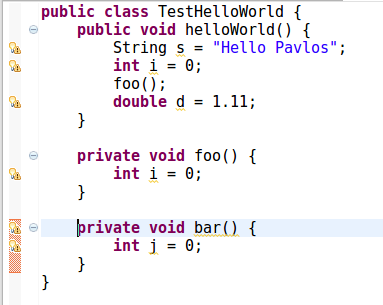
\includegraphics[width=.6\linewidth]{figures/Selection_078}
	\caption[A sample Java program]{\label{f:sampProg}A sample Java program.}
\end{figure}

\begin{figure}[ht]
	\centering
	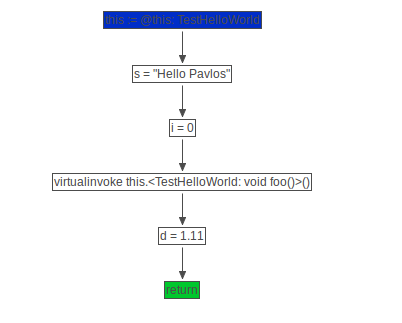
\includegraphics[width=.6\linewidth]{figures/Selection_079}
	\caption[The PDG of the sample Java program in Figure~\ref{f:sampProg}]{\label{f:sampPdg}The PDG of the sample Java program in Figure~\ref{f:sampProg}.}
\end{figure}

\subsection{Information flow sets}

Soot provides a very useful feature to its built in PDGs, which is the ability to create so called in/out flow sets within a node in the graph as shown in Figure~\ref{f:sampInOut}, of which is essentially just the information known to a node upon entry and exit.

This is one of the key points to note with our SDG implementation; in flow set information can be used by a function call as argument parameters, and upon return of the function, the out flow set may be modified by it, assuming a single threaded application is being analyzed (see Section 3.1).

\begin{figure}[ht]
	\centering
	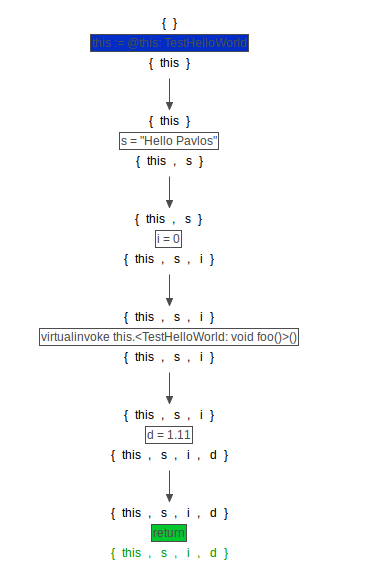
\includegraphics[width=.6\linewidth]{figures/Selection_080}
	\caption[A PDG with in/out flow information denoted.]{\label{f:sampInOut}A PDG with in/out flow information denoted.}
\end{figure}


\section{Implementation and Results}

We now discuss our approach to implement SDGs using Soot PDGs. As mentioned previously, SDGs are essentially, in their simplest form, just multiple PDGs coalesced together. We take note of the fact that Soot marks function invocations via \textit{virtualinvoke} tags and use this as the entry and exit points for spawning the additional PDGs.

\subsection{Key assumptions}

One of the key assumptions that were made for our implementation is that the Java programs that will be analyzed are synchronous. Threaded applications give rise to major difficulties as the in/out flow set information within nodes are compromised and may not be accurate depending on how the threading is performed. For strictly academic purposes we decided that this was an unnecessary complication.

Another assumption is that the Java programs to be analyzed will only have Java primitives as their contents. There are significant bugs present in the Soot framework, one of them being that the PDG cannot be generated if there are library method calls in the body of the function, such as \textit{System.out.println()}, among others. We attributed this to a Soot limitation, and as such, chose to ignore it for our purposes.

Lastly we also assume a forward non-branched analysis, i.e. the function cannot flow between one of several divergent paths that would be introduced by an \textit{if} statement, for example. Again, this introduces needless complications, and since this is a purely academic exercise, we chose to ignore this case. Soot however provides a \textit{forward branched flow analysis} of which should be investigated in the future as this would handle said limitation.

\subsection{Base case: direct function call}

To handle the simplest case of a direct function call, we make use of Soot \textit{virtualinvoke} tags to detect when an occurrence takes place. In such an event, a new PDG is spawned, alongside the original PDG, which represents the control flow information for the invoked function as shown in Figure~\ref{f:firstImpl}. Due to time constraints, several bugs persists, the main one being the apparent lack of edges between the entry and exit points of the additional function call.

\begin{figure}[ht]
	\centering
	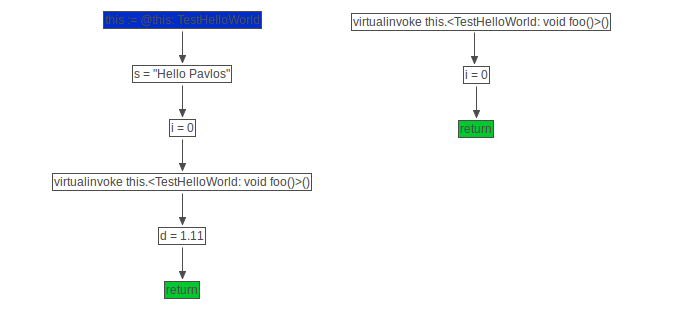
\includegraphics[width=.6\linewidth]{figures/Selection_083}
	\caption[An SDG for the simplest case: a direct function call.]{\label{f:firstImpl}An SDG for the simplest case: a direct function call..}
\end{figure}

\subsection{Additional cases: recursion and lambda functions}

Due to time constraints this aspect of the project was not able to be completed.

\section{Conclusion}

SDGs are superior to PDGs because it allows one to model information arising from inter-procedural method flows. SDGs thus are able to improve program optimization and slicing tasks by providing more information than ordinarily present with just PDGs, at the cost of increased complexity. We discussed our attempts at implementing an SDG via the Soot framework, of which is able to generate PDGs out of the box, but not SDGs. Most analysis frameworks are not able to provide SDGs due to their novel nature; this is the primary motivating factor behind this project, as an SDG is a highly advantageous form of a PDG. While we were able to implement the simplest case, which would be a direct function call within a method, we were not able to handle more complex cases, such as recursion and lambda functions, due to time constraints. It should be investigated in the future whether this is possible with the Soot framework, as in doing so would remove the major limitations of this project.

\bibliographystyle{abbrvnat}
\bibliography{references}


\bibliographystyle{abbrvnat}



\end{document}
